\chapter{Système de Maintenance automatisé}
Le 1er modèle est un système contenant deux machines $M_1$ et $M_2$ dont la maintenance doit être assurée car celles-ci peuvent tomber en pannes. Pour représenter notre système à commander, nous avons pris comme représentation de  $M_1$ et $M_2$ les automates :
\begin{center}
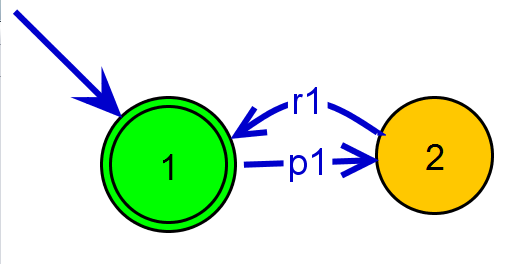
\includegraphics[scale=0.3]{I/images/M1.png}
\captionof{figure}{Machine $M_1$}
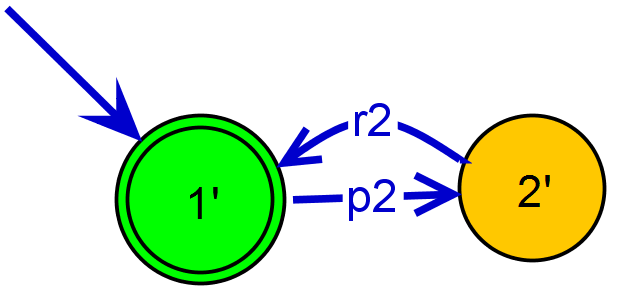
\includegraphics[scale=0.3]{I/images/M2.png}
\captionof{figure}{Machine $M_2$}
\end{center}
où : \begin{itemize}[label = \textbullet]
\item $p_1$ et $p_2$ sont les pannes sur les machines $M_1$ et $M_2$.
\item $r_1$ et $r_2$ sont les réparations sur les machines $M_1$ et $M_2$.
\end{itemize}


Nous avons obtenu le modèle $P$, soit le produit parallèle entre $M_1$ et $M_2$ (EXPLICATION) suivant à l'aide de DESUMA : 
\begin{center}
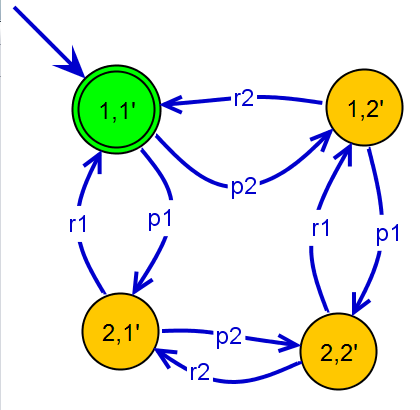
\includegraphics[scale=0.5]{I/images/P.png}
\captionof{figure}{Modèle automate $P$}
\end{center}
Nous utilisons le produit parallèle pour obtenir un automate qui laisse toutes les possibilités d'évolution à $M_1$ et $M_2$. Or, le système complet $P$, en supposant que $M_1$ et $M_2$ sont indépendants, permet de présenter toutes les évolutions de $M_1$ et de $M_2$ tel que : $P = \Sigma(M_1)\ U\ \Sigma(M_1)$.

Nous obtenons le modèle des spécifications $S_1$ suivant :\\
\begin{center}
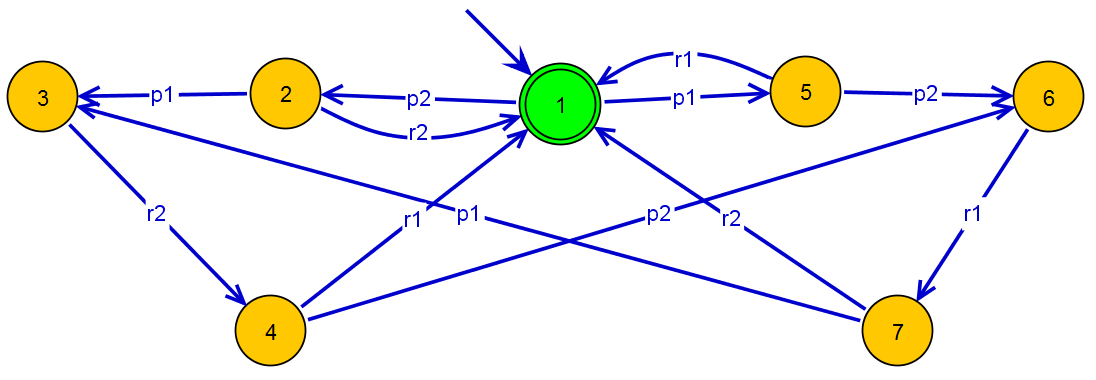
\includegraphics[scale=0.5]{I//images/S1.png}
\captionof{figure}{Modèle automate $S$}
\end{center}dans lequel nous relevons les propriétés suivantes :
\begin{itemize}[label = \textbullet]
\item Spécification totale car les langages de $S_1$ et de $P$ sont identiques : $\Sigma_{S_1} = \Sigma_P$
\item Spécification dynamique car notre automate $S_1$ représente les séquences d'évènements autorisées.
\end{itemize}

Notre modèle de spécifications nous amène donc à la commande supervisé suivante :\begin{center}

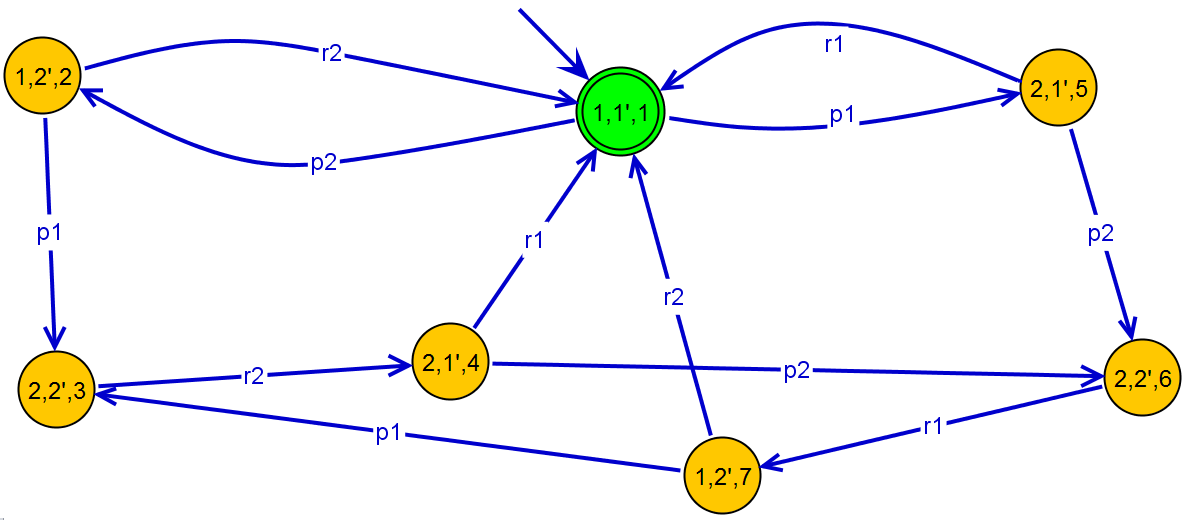
\includegraphics[scale=0.3]{I/images/P_S1.png}
\captionof{figure}{Modèle de commande supervisé $P/S_1$}

\end{center}construit à l'aide du produit parallèle car la spécification est partielle.
A l'aide de DESUMA, nous avons pu vérifier la propriété de commandabilité de notre automate de commande supervisé, nous sommes donc capable d'affirmer qu'aucun évènements non contrôlable ne va causer des séquences non définis par $S_1$.
\begin{center}
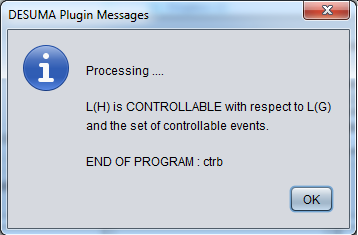
\includegraphics[scale=0.5]{I/images/P_S1_ctrbl.png}
\captionof{figure}{Message DESUMA}
\end{center}
Pour vérifier le non blocage de notre commande supervisé, nous allons vérifier que chaque état de $P/S_1$ est co-accessible, ce qui revient à déterminer si chaque état peut accéder à l'état marqué. Ce état est la paire (1,1), et nous constatons que touts les autres paire $(x_P,x_S)$ ont accès via une séquence la paire d'états marqués. La commande obtenue est donc non bloquante ce qui conclut notre première étude de cas. 